%% 07_model3_macro_transmission.tex
%% Section 7: Model 3 -- Macro-Financial Transmission

\section{Model 3: Macro-Financial Transmission}
\label{sec:model3}

The third model aggregates the firm-level and bank-level results from Models 1 and 2 into a macro-financial impact assessment. We decompose the total GDP effect of coal stranding into three channels (fiscal, credit, and market) and estimate their magnitudes using an accounting framework calibrated to Indonesian macroeconomic parameters.

\subsection{Three-Channel Framework}
\label{subsec:three_channel}

Our conceptual framework, illustrated in Figure~\ref{fig:conceptual}, identifies three transmission channels through which coal stranding affects aggregate output:

\begin{figure}[htbp]
\centering
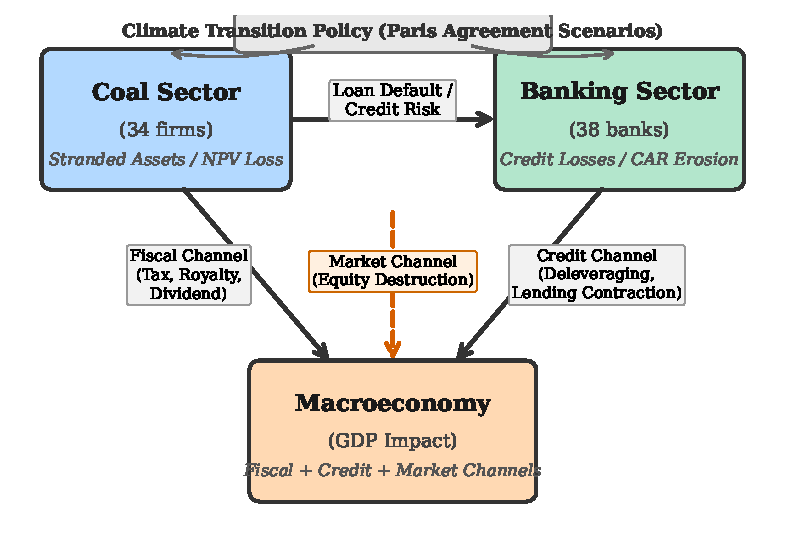
\includegraphics[width=\textwidth]{figures/fig_01.pdf}
\caption{Conceptual framework: the coal-banking-sovereign nexus. Coal stranding transmits to the macroeconomy through three channels: fiscal (government revenue loss), credit (bank deleveraging), and market (equity value destruction). Arrows indicate direction of transmission; dashed lines indicate feedback effects not modelled in our framework.}
\label{fig:conceptual}
\end{figure}

\begin{enumerate}
\item \textbf{Fiscal channel}: Reduced coal production and profitability lower government revenues from corporate taxes, royalties, and state-owned enterprise dividends, necessitating either fiscal consolidation or increased borrowing.

\item \textbf{Credit channel}: Bank credit losses from coal exposures deplete bank capital, triggering a deleveraging response that reduces credit supply to the broader economy, with multiplier effects on investment and consumption.

\item \textbf{Market channel}: The destruction of equity value in coal companies and exposed banks reduces household and institutional wealth, dampening consumption and investment through the wealth effect.
\end{enumerate}

The total GDP impact is the sum of the three channel-specific effects:
\begin{equation}
\label{eq:total_gdp}
\Delta GDP^s = \Delta GDP^{fiscal,s} + \Delta GDP^{credit,s} + \Delta GDP^{market,s}
\end{equation}

We calibrate the framework to Indonesia's macroeconomic context, using a nominal GDP of \$1,319 billion (2023) as the base.

\subsection{Fiscal Channel}
\label{subsec:fiscal_channel}

The fiscal impact arises from three sources of government revenue loss: corporate income tax, mining royalties, and dividends from PT Bukit Asam (PTBA), the state-owned coal company.

\subsubsection{Corporate Tax Loss}

Under scenario $s$, the revenue decline for coal company $i$ relative to BAU reduces corporate tax payments:
\begin{equation}
\label{eq:tax_loss}
\Delta Tax^s = \sum_{i} \left(R_i^{BAU} - R_i^s\right) \times \tau
\end{equation}
where $R_i^{BAU}$ and $R_i^s$ are firm revenues under BAU and scenario $s$, respectively, and $\tau = 0.22$ is the corporate tax rate. The revenue decline under each scenario is estimated by scaling current revenues by the ratio of scenario to BAU coal prices at the 2030 horizon: $R_i^s = R_i^{current} \times (P^s_{2030} / P^{BAU}_{2030})$.

\subsubsection{Royalty Loss}

Indonesia's coal royalty system charges between 3\% and 7\% of the sales value depending on coal type and contract terms. We apply each firm's specific royalty rate (from the operational template data) to the revenue decline:
\begin{equation}
\label{eq:royalty_loss}
\Delta Royalty^s = \sum_{i} \left(R_i^{BAU} - R_i^s\right) \times \rho_i
\end{equation}
where $\rho_i$ is the firm-specific royalty rate.

\subsubsection{PTBA Dividend Loss}

As a state-owned enterprise, PTBA pays dividends to the government. We estimate the dividend loss proportional to the revenue decline:
\begin{equation}
\label{eq:dividend_loss}
\Delta Div^s = Div^{current}_{PTBA} \times \frac{P^{BAU}_{2030} - P^s_{2030}}{P^{BAU}_{2030}}
\end{equation}

\subsubsection{Fiscal GDP Impact}

The total fiscal loss is translated into GDP impact through the fiscal multiplier:
\begin{equation}
\label{eq:fiscal_gdp}
\Delta GDP^{fiscal,s} = \left(\Delta Tax^s + \Delta Royalty^s + \Delta Div^s\right) \times \mu_{fiscal} / GDP
\end{equation}
where $\mu_{fiscal} = 0.70$ is the fiscal multiplier, conservatively calibrated based on estimates for Indonesia and comparable emerging economies. The fiscal multiplier reflects the fact that a dollar of lost government revenue does not translate one-for-one into lost output, as the government may partially offset the shortfall through borrowing or expenditure reallocation.

Under the 2\textdegree C scenario, the total fiscal loss amounts to \$1,318 million (tax: \$1,023M, royalty: \$263M, PTBA dividend: \$33M), generating a GDP impact of 0.070\%. Under the 1.5\textdegree C scenario, the fiscal loss rises to \$2,197 million, with a GDP impact of 0.117\%.

\subsection{Credit Channel}
\label{subsec:credit_channel}

The credit channel operates through the bank lending mechanism. When banks suffer credit losses from coal exposures, they must either raise new capital or reduce their balance sheets to restore capital adequacy ratios. In practice, deleveraging (reducing the loan book) is the more common response, particularly during periods of stress when new capital issuance is costly.

The credit contraction for bank $b$ is estimated using a leverage multiplier:
\begin{equation}
\label{eq:credit_contraction}
\Delta Credit_b^s = L_b^s \times \kappa
\end{equation}
where $L_b^s$ is the bank's total credit loss from Model 2 and $\kappa = 8$ is the credit multiplier, reflecting the average leverage ratio of Indonesian banks (approximately 8:1 assets to equity). This multiplier captures the mechanical relationship between capital depletion and lending capacity: a \$1 loss of capital necessitates an \$8 reduction in risk-weighted assets to maintain the same CAR.

The aggregate credit contraction is translated into GDP impact through the credit-GDP elasticity:
\begin{equation}
\label{eq:credit_gdp}
\Delta GDP^{credit,s} = \frac{\sum_b \Delta Credit_b^s}{GDP} \times \varepsilon_{credit}
\end{equation}
where $\varepsilon_{credit} = 0.06$ is the credit-to-GDP elasticity, estimated from the empirical relationship between credit growth and GDP growth in Indonesia over the 2010--2023 period. This parameter implies that a 1 percentage point reduction in credit-to-GDP translates to a 0.06 percentage point reduction in GDP growth, consistent with estimates from \citet{GambacortaMarques2011} for bank-dependent economies.

Under the 2\textdegree C scenario, the aggregate credit contraction is \$14.8 billion (3.20\% of total bank credit), generating a GDP impact of 0.192\%. Under the 1.5\textdegree C scenario, the contraction increases to \$25.2 billion (5.45\%), with a GDP impact of 0.327\%. The credit channel is the dominant transmission mechanism, accounting for approximately 60\% of the total GDP impact under both scenarios.

\subsection{Market Channel}
\label{subsec:market_channel}

The market channel captures the wealth effect from equity value destruction in coal companies and exposed banks. We estimate market capitalisation losses for both sectors:

\subsubsection{Coal Equity Losses}

For each coal company, the equity value destruction is proportional to the NPV decline:
\begin{equation}
\label{eq:coal_mktcap}
\Delta MktCap_i^{coal,s} = MktCap_i \times \frac{NPV_i^{BAU} - NPV_i^s}{NPV_i^{BAU}}
\end{equation}

Under the 2\textdegree C scenario, aggregate coal equity losses amount to \$24.2 billion. Under the 1.5\textdegree C scenario, these losses reach \$37.0 billion.

\subsubsection{Bank Equity Losses}

Bank equity losses are estimated using a coal-sector beta that captures the sensitivity of bank valuations to coal sector performance:
\begin{equation}
\label{eq:bank_mktcap}
\Delta MktCap_b^{bank,s} = MktCap_b \times \beta_{b,coal} \times \frac{\Delta CoalIndex^s}{CoalIndex}
\end{equation}
where $\beta_{b,coal}$ is estimated from the bank's coal exposure as a share of total assets. Under the 2\textdegree C and 1.5\textdegree C scenarios, aggregate bank equity losses amount to \$2.1 billion and \$3.8 billion, respectively.

\subsubsection{Market GDP Impact}

The total market capitalisation loss is translated into GDP impact through the wealth effect:
\begin{equation}
\label{eq:market_gdp}
\Delta GDP^{market,s} = \frac{\Delta MktCap_{total}^s \times \mu_{wealth}}{GDP}
\end{equation}
where $\mu_{wealth} = 0.03$ is the marginal propensity to consume out of wealth, a conservative estimate for Indonesia where equity market participation is lower than in advanced economies. Under the 2\textdegree C scenario, the market channel generates a GDP impact of 0.060\%; under 1.5\textdegree C, the impact is 0.093\%.

\subsection{Aggregate Impact}
\label{subsec:aggregate_impact}

Table~\ref{tab:macro_impact} summarises the macro-financial impact across all three channels and both climate scenarios.

\begin{table}[htbp]
\centering
\caption{Macro-Financial Impact of Coal Stranded Assets}
\label{tab:macro_impact}
\footnotesize
\begin{tabular}{lrrrr}
\toprule
 & \multicolumn{2}{c}{2\textdegree{}C Paris} & \multicolumn{2}{c}{1.5\textdegree{}C NZE} \\
\cmidrule(lr){2-3} \cmidrule(lr){4-5}
Channel & Loss (\$M) & GDP (\%) & Loss (\$M) & GDP (\%) \\
\midrule
  \textit{Fiscal channel} & & & & \\
  \quad Corporate tax loss & 1,005.4 & 0.053\% & 1,675.6 & 0.089\% \\
  \quad Royalty loss & 258.7 & 0.014\% & 431.2 & 0.023\% \\
  \quad PTBA dividend loss & 32.6 & 0.002\% & 54.3 & 0.003\% \\
  \quad \textit{Fiscal subtotal} & \textit{1,296.7} & \textit{0.069\%} & \textit{2,161.1} & \textit{0.115\%} \\[4pt]
  \textit{Credit channel} & & & & \\
  \quad Bank deleveraging & 14,463.1 & 0.188\% & 25,292.5 & 0.328\% \\
  \quad \textit{Credit subtotal} & \textit{14,463.1} & \textit{0.188\%} & \textit{25,292.5} & \textit{0.328\%} \\[4pt]
  \textit{Market channel} & & & & \\
  \quad Coal equity loss & 48,060.9 & 0.109\% & 75,199.2 & 0.171\% \\
  \quad Bank equity loss & 2,347.8 & 0.005\% & 4,189.8 & 0.010\% \\
  \quad \textit{Market subtotal} & \textit{50,408.7} & \textit{0.115\%} & \textit{79,389.1} & \textit{0.181\%} \\[4pt]
  \textbf{Total GDP impact} & & \textbf{0.371\%} & & \textbf{0.624\%} \\
\bottomrule
\end{tabular}

\smallskip
\noindent \textit{Notes:} GDP impact estimated via three transmission channels. Fiscal: lost corporate tax (22\% rate), royalties, and PTBA state dividends. Credit: bank deleveraging multiplied by credit-to-GDP multiplier (8$\times$). Market: decline in coal and bank equity market capitalization, transmitted via wealth effect (0.03 MPC). GDP denominator: Indonesia 2024 nominal GDP at current prices. Sample: 26 coal companies with verified production and cost data (ADRO excluded following 2024 restructuring; see Section~\ref{subsec:coal_data}).
\end{table}


Under the 2\textdegree C scenario, the total GDP impact is 0.32\%, decomposed as fiscal (0.070\%), credit (0.192\%), and market (0.060\%). Under the 1.5\textdegree C scenario, the total impact rises to 0.54\%, with the credit channel (0.327\%) remaining the dominant contributor, followed by the fiscal channel (0.117\%) and the market channel (0.093\%).

Figure~\ref{fig:waterfall} presents a waterfall diagram illustrating the cumulative build-up of GDP impact across channels under the 1.5\textdegree C scenario.

\begin{figure}[htbp]
\centering
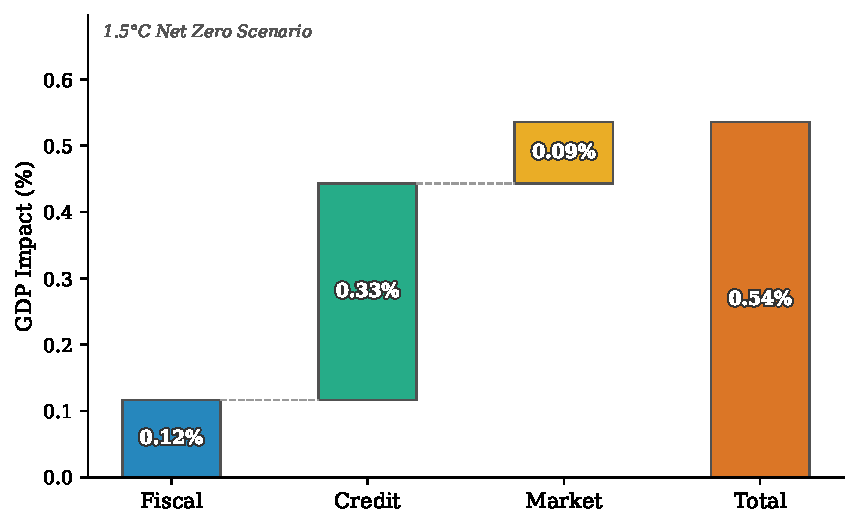
\includegraphics[width=\textwidth]{figures/fig_09.pdf}
\caption{Waterfall diagram of GDP impact under the 1.5\textdegree C scenario. Each bar represents the incremental contribution of a transmission channel: fiscal (tax, royalty, and PTBA dividend), credit (bank deleveraging), and market (coal and bank equity destruction). The rightmost bar shows the total cumulative impact of 0.54\% of GDP.}
\label{fig:waterfall}
\end{figure}

Several observations are warranted. First, the dominance of the credit channel reflects Indonesia's bank-dependent financial structure, where bank lending is the primary source of external finance for the corporate sector. This finding aligns with \citet{PeekRosengren2000} and \citet{GambacortaMarques2011}, who demonstrate that credit channel effects are amplified in economies with limited capital market alternatives. Second, the market channel impact, while substantial in absolute terms, is attenuated by the relatively low equity market participation rate in Indonesia (approximately 4\% of the population holds equity directly), which limits the consumption wealth effect. Third, our fiscal impact estimate is likely conservative, as it excludes second-round effects such as reduced investment in coal-dependent regions, lower personal income tax revenues from displaced mining workers, and potential sovereign credit rating implications.
